%##noBuild
\newpage
\section{Polecenie 6}

\subsection{ZMIEN STATUS REZERWACJI ORAZ TABELA REZERWACJE LOG}
Dodajemy tabelę dziennikującą zmiany statusu rezerwacji
rezerwacje\_log(id, id\_rezerwacji, data, status)
Należy zmienić warstwę procedur modyfikujących dane tak aby dopisywały informację do
dziennika. Przez pomyłkę zaimplementowałem nazwę dziennik\_rezerwacji zamiast rezerwacje\_log. 
Mam nadzieję że nie stanowi to problemu.

\subsubsection{TABELA DZIENNIK REZERWACJI}
\begin{verbatim}
CREATE TABLE DZIENNIK_REZERWACJI
(
ID_ZMIANY_STATUSU INT GENERATED ALWAYS AS IDENTITY NOT NULL
, NR_REZERWACJI INT
, DATA DATE
, NOWY_STATUS CHAR
, CONSTRAINT DZIENNIK_REZERWACJI_PK PRIMIARY KEY
 (
 ID_ZMIANY_STATUSU
 )
 ENABLE
);
\end{verbatim}

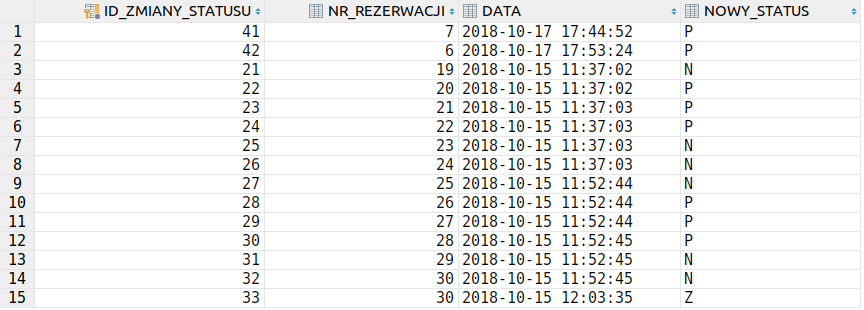
\includegraphics[width=\linewidth]{./images/tabela_dziennik_rezerwacji.png}

\subsubsection{ZMIEN STATUS REZERWACJI}
\begin{verbatim}
CREATE OR REPLACE PROCEDURE ZMIEN_STATUS_REZERWACJI_2(ID_REZERWACJI NUMBER, NOWY_STATUS_ CHAR)
AS
  BEGIN
    DECLARE
      ID_R            NUMBER;
      S               CHAR;
      DZISIEJSZA_DATA DATE;
    BEGIN
      SELECT COUNT(R.NR_REZERWACJI) INTO ID_R FROM REZERWACJE R WHERE R.NR_REZERWACJI = ID_REZERWACJI;
      SELECT R.STATUS INTO S FROM REZERWACJE R WHERE R.NR_REZERWACJI = ID_REZERWACJI;
      SELECT CURRENT_DATE INTO DZISIEJSZA_DATA FROM DUAL;
      IF ID_R = 1
      THEN
        IF (S <> 'A') AND NOWY_STATUS_ IN ('N', 'P', 'Z') AND NOWY_STATUS_ <> S
        THEN
          UPDATE REZERWACJE R SET R.STATUS = NOWY_STATUS_ WHERE R.NR_REZERWACJI = ID_REZERWACJI;
          INSERT INTO DZIENNIK_REZERWACJI (NR_REZERWACJI, DATA, NOWY_STATUS)
          VALUES (ID_REZERWACJI, DZISIEJSZA_DATA, NOWY_STATUS_);
        END IF;
      END IF;
    END;
  END;
\end{verbatim}

Po wykonaniu procedury:
\begin{verbatim}
begin
  ZMIEN_STATUS_REZERWACJI_2(6, 'Z');
end;
\end{verbatim}

Następuje zmiana statusu rezerwacji dla rezerwacji o id = 6 i zostaje to zapisane do dziennika rezerwacji.

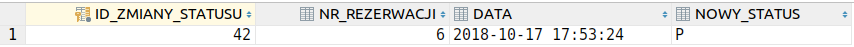
\includegraphics[width=\linewidth]{./images/zmien_status_rezerwacji_2.png}
